\section{Evaluation}
\label{sec:eval}

\begin{figure*}[ht]
    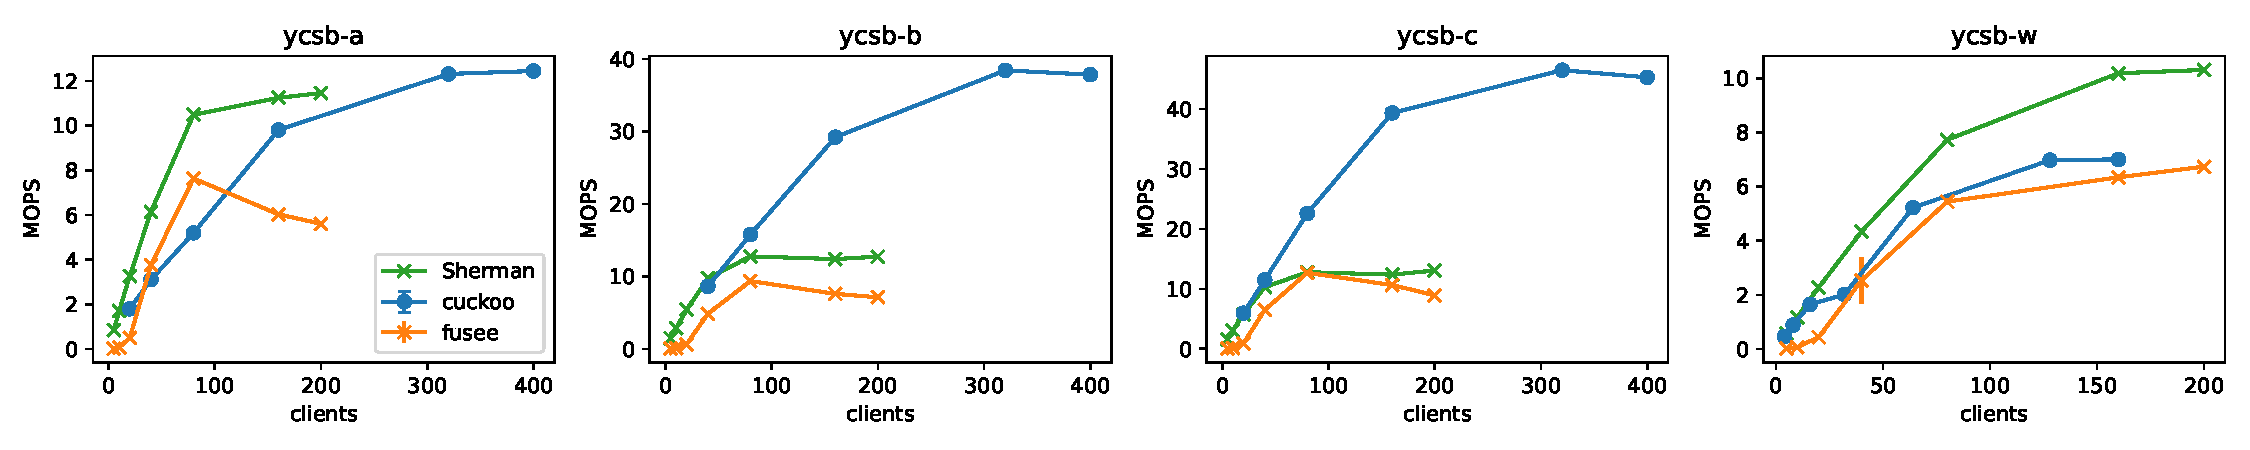
\includegraphics[width=0.99\linewidth]{fig/hero_ycsb_throughput.pdf}
    \caption{race vs rcuckoo simulated throughput \todo{rerun ycsb-b numbers don't look quite right}}
    \label{fig:ycsb_throughput}
\end{figure*}

\begin{figure*}[ht]
    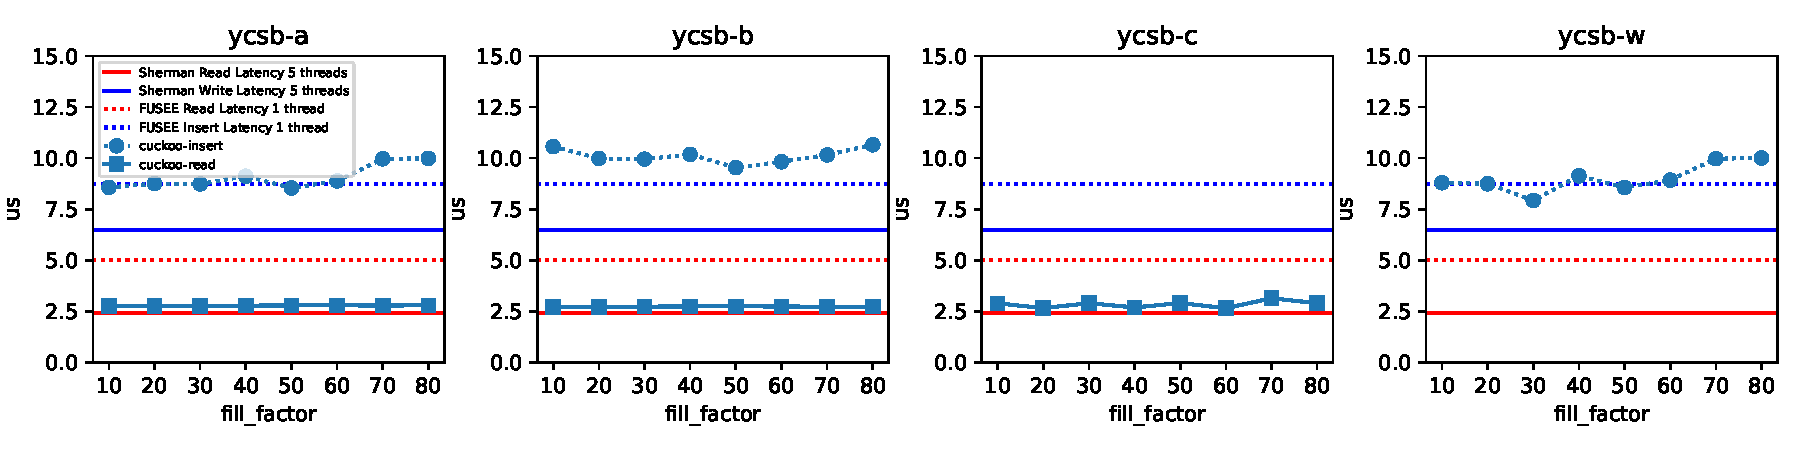
\includegraphics[width=0.99\linewidth]{fig/hero_ycsb_fill_latency.pdf}
    \caption{race vs rcuckoo workload fill latency}
    \label{fig:ycsb_fill_latency}
\end{figure*}

\begin{figure}[ht]
    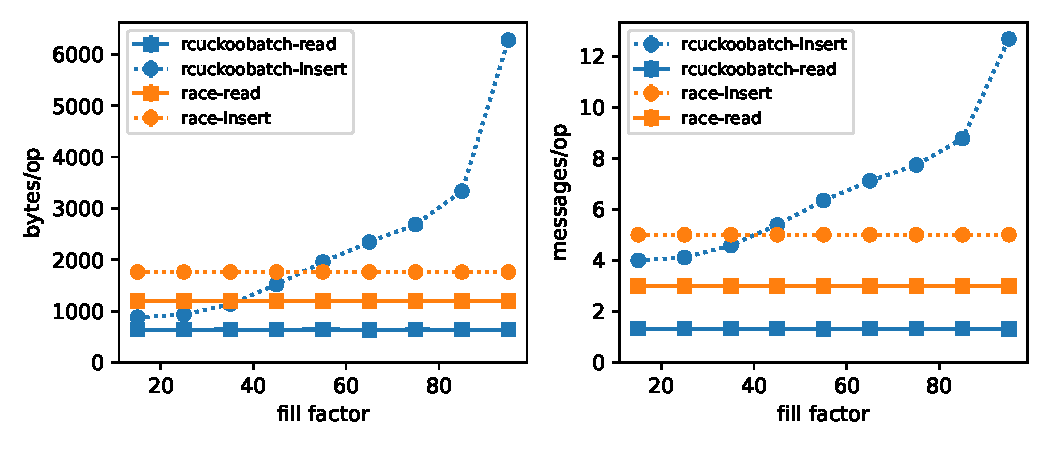
\includegraphics[width=0.99\linewidth]{fig/hero_ycsb_fill_ops_bw.pdf}
    \caption{YCSB-A workload messages and bandwidth per operation as a function of fill factor}
    \label{fig:ycsb_fill_ops_bw}
\end{figure}

\begin{figure}[ht]
    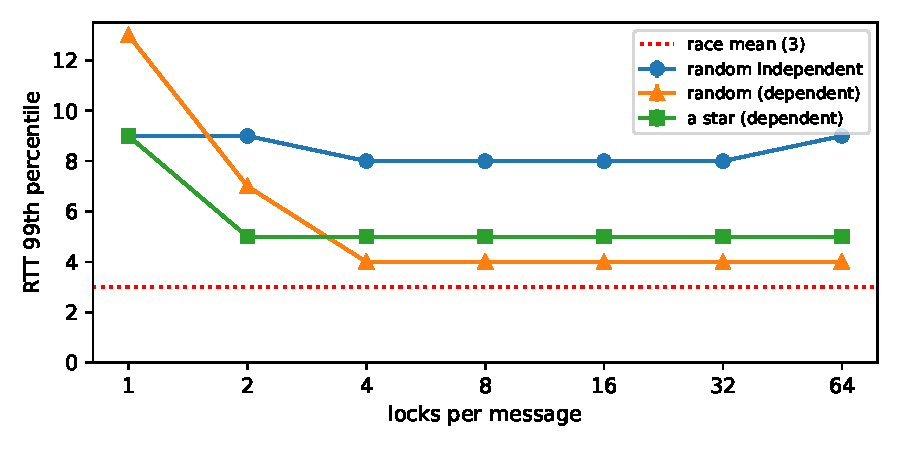
\includegraphics[width=0.99\linewidth]{fig/search_dependence.pdf}

    \caption{Round trips per insert operation compared
    across search functions and hash functions. Dependent
    hash functions with A* have the shortest search
    times.~\todo{latest numbers for A* are counter intuitive
    - dig into}}

    \label{fig:search_dependence}
\end{figure}

Our evaluation is run entirely in simulation. The goal of
our evaluation is to demonstrate the practicality of rcuckoo
by showing through simulation that it supports low latency
and high throughput operations. We measure blocking round
trips as a proxy for latency. To approximate throughput we
measure the total number of blocking round trips required to
fill the table, and divide by the number of concurrent
clients. All of our evaluations are carried out on hash
tables with buckets of size 8, and key-value pairs with
32bit keys and 16bit values. On hash tables with 1 million
entries. Rcuckoo is set with a read threshold of 512 bytes.

In each experiment clients operate on a shared remote hash
table, but insert and read independent sets of keys. Using
independent keys prevents clients from reading absent keys,
and inserting duplicate keys.  However it does not prevent
interference due to hash collisions or conflicting cuckoo
paths.


\subsection{System Performance}

\textbf{Throughput:} Figure~\ref{fig:ycsb_throughput} shows
the throughput of RACE vs rcuckoo for YCSB workloads. YCSB-W
is a 100\% write workload. YCSB-A is a 50\% read 50\% write
workload. YCSB-B is 95\% read and 5\% write, and YCSB-C is
100\% read.  In each experiment clients fill the hash table
from empty to 90\% full. For read only workloads the hash
table is first filled to 90\% and then clients read from the
table.  Note that on large tables rcuckoo inserts scale
almost linearly as the number of path collisions on inserts
remains low due to the short cuckoo range.  Read heavy
workloads (ycsb-b, c) have the highest throughput due to
fewer round trips. In the case of ycsb-c rcuckoo achieves 2x
the read throughput of RACE.

\textbf{Latency:} Rcuckoo's operation latency is not static
across fill factors. Because cuckoo paths are likely to be
longer at higher table saturations inserts are more likely
to require more round trips when obtaining locks. We measure
the round trips as a proxy for latency at incremental fill
factors. In each experiment the table is filled to the
specified fill factor and requests are executed until the
table reaches an additional 5\% fill or in the case of read
only 500k. Each experiment is run with 128 clients.
requests are issued. 
%%
Figure~\ref{fig:ycsb_fill_latency}, shows the average
operation latency for each workload. Here average RTT is the
average between both reads and writes. RACE incurs
additional round trips from reading from its extent and
from verifying its successful inserts. RACE has very few
collisions as its critical section for insertion is the
duration of a single RDMA CAS. Few of RACE's inserts fail
and it retains near constant latency for read and writes
across all fill factors. The same is true for rcuckoo reads
which remain at a single round trip. Rcuckoo inserts are
subject to additional round trips as the table fills.  Most
additional round trips are caused by locks being spaced
further than the span of an RDMA CAS on the lock table. Some
are caused by contention. The small improvement of ycsb-a
and ycsb-b over ycsb-w inserts are due to reduced write
contention from the workload.

\textbf{Bandwidth, and messages:} Rcuckoo design trades off
bandwidth for latency by increases the size of reads for all
operations. We measure the effect of fill factor on the
bandwidth and messages required per operation with the same
experiment used to measure latency.
Figure~\ref{fig:ycsb_fill_ops_bw} shows how rcuckoo and
RACE's messages and bandwidth respond to fill factor. At low
fill rates (less than 50\%) rcuckoo uses less bandwidth per
operation and less messages per operation than RACE. Above
50\% collisions in the hash table increase the cost of
insertions. While the size of the cuckoo path does not
directly relate to the number of round trips, it does
directly relate to messages. High fill factors nearly double
the number of insert messages required to perform insertions
with rcuckoo, and bandwidth can increase by up to a factor of
4. \todo{In the future we could perform very large writes to
reduce the number of messages at the cost of more
bandwidth.}

\textbf{Locks per message and independence:} Hash function
locality hash a major impact in rcuckoo's performance.
Acquiring locks can only be done in a few round trips when
the locks are clustered together tightly in the lock table.
Furthermore, the search function used to determine the
cuckoo path has a large impact on the locality of the locks
necessary to lock the path. We evaluate dependent hashing
and independent hashing as well as random and a* search. We
measure the number of round trips required for each control
as a function of the number of locks which can be acquired
per round trip.

Figure~\ref{fig:search_dependence} shows the performance
improvements gained by both locality hashing and A* search.
In this experiment the table is filled from 0 to 90\% full
with a ycsb-w workload. We measure the 99th percentile of
round trips for these workloads. Random search with
independent hashing leads to a large number of round trips
as locks are scattered throughout the table. RDMA masked CAS
operation do little here to reduce the round trips as they
can rarely aquire more than one lock in a round trip. With
dependent hashing and random search RDMA CAS operation are
almost sufficient to reduce round trips, however the absolute
number of locks required per insert is high which leads to
greater contention. A* search with dependent hashing has
cuckoo paths that are both short, and clustered together.



\subsection{Search Performance:}

\todo{\textbf{A* search vs BFS:} We compare the performance of A*
vs BFS for locally computed insertions. A* performance
directly effects system throughput as this algorithm is run
twice on every insert.}

\todo{\textbf{Hashing Algoritms:} Rcuckoo hashing requires
executing many hash compuations. We evaluate our A* search
alorithm abolute performacne on various hash functions and
show how this values effect our overall fill factors.}

\subsection{Read Threshold Performance} 

\todo{Show how it reduces messages per operation. This is not that
important of an experiment as I can't show the latency
overhead of two batched messages vs one at the moment.}
%%